%%%%%%%%%%%%%%%%%%%%%%%%%%%%%%%%%%%%%%%%%%%%%%%%%%%%%%%%%%%%%%%%%%%%%%%%%%%%%%%%
%%%%%%%%%%%%%%%%%%%%%%%%%%%%%%%%%%%%%%%%%%%%%%%%%%%%%%%%%%%%%%%%%%%%%%%%%%%%%%%%
\documentclass[11pt]{article}

\usepackage[numbers,square]{natbib}
\renewcommand\cite[1]{(\citet{#1})}
\usepackage
[
        a4paper,% other options: a3paper, a5paper, etc
        left=2cm,
        right=2.5cm,
        top=3cm,
        bottom=4cm,
        % use vmargin=2cm to make vertical margins equal to 2cm.
        % us  hmargin=3cm to make horizontal margins equal to 3cm.
        % use margin=3cm to make all margins  equal to 3cm.
]
{geometry}
\usepackage{color}
\usepackage{chemarr}
\usepackage{amssymb}
\usepackage{graphicx}
\usepackage{textcomp} 
\usepackage[gen]{eurosym}
\usepackage{amsmath}
\usepackage[margin=1.5cm]{caption}
\usepackage{amsmath,mathtools}
\usepackage{subcaption}
%\setlength{\belowcaptionskip}{-5pt}
%\setlength{\abovecaptionskip}{-8pt}
\usepackage{enumitem}

%\usepackage[autolinebreaks,useliterate]{mcode}
\usepackage[usenames, dvipsnames]{xcolor}
\colorlet{shadecolor}{gray!5}
\usepackage{listings}
\lstset{ 
  language=R,                     % the language of the code
  basicstyle=\scriptsize\ttfamily, 	  % the size of the fonts
  numbers=left,                   % where to put the line-numbers
  numberstyle=\tiny\color{Blue},  % the style that is used for the line-numbers
  stepnumber=1,                   % the step between two line-numbers.
  numbersep=5pt,                  % how far the line-numbers are from the code
  backgroundcolor=\color{shadecolor},  % choose the background color.
  showspaces=false,               % show spaces adding particular underscores
  showstringspaces=false,         % underline spaces within strings
  showtabs=false,                 % show tabs within strings adding particular underscores
  frame=tb,                   	  % adds a frame around the code
  rulecolor=\color{Black},        % if not set, the frame-color may be changed on line-breaks within not-black text (e.g. commens (green here))
  tabsize=2,                      % sets default tabsize to 2 spaces
  captionpos=b,                   % sets the caption-position to bottom
  breaklines=true,                % sets automatic line breaking
  breakatwhitespace=false,        % sets if automatic breaks should only happen at whitespace
  keywordstyle=\color{RoyalBlue}, % keyword style
  commentstyle=\color{OliveGreen},% comment style
  stringstyle=\color{ForestGreen} % string literal style
}



%%%%%%%%%%%%%%%%%%%%%%%%%%%%%%%%%%%%%%%%%%%%%%%%%%%%%%%%%%%%%%%%%%%%%%%%%%%%%%%%
\title{\textbf{Mass Fraction of BC in 90 - 400 nm} \\ 
\textbf{(For Comparison with SP2 Measurements)}}
\author{Yinrui Li}
\date{}


%\maketitle


\begin{document}
\maketitle
%%%%%%%%%%%%%%%%%%%%%%%%%%%%%%%%%%%%%%%%%%%%%%%%%%%%%%%%%%%%%%%%%%%%%%%%%%%%%%%%



\section{SP2 Measurement} 

The measurement range of the SP2 instrument is approximately 90 $\sim$ 400 nm BC diametet, which is unlikely to represent the total ambient number and mass concentrations of BC (Reddington et al., 2013). In order to compare CAMChem model simulated BC with observations, we estimated the mass fraction of modeled BC in the size range (90 $\sim$ 400 nm) corresponding to SP2 measurement.


 
\section{Estimating the mean BC core diameter in primary carbon mode and in accumulation mode} 

A 4-mode version of the modal aerosol model (MAM4) is applied in CAMChem1.2.2. BC is emitted to the primary carbon mode, and then is aged and transferred to the accumulation mode by condensation of $\rm{H_2SO_4}$, $\rm{NH_3}$ and $\rm{SOA}$ and by coagulation (Liu et al., 2012). In primary carbon mode, particles consist of externally mixed BC and OC, whereas in accumulation mode, particles consist of internally mixed BC and non-BC material.
\bigskip
\noindent SP2 measures the mass size distribution of the BC particle cores over a calibrated volume equivalent diameter (VED) range of 55 to 400 nm, and the number-detection efficiency at sea level pressure is reported to be one for BC above 90 nm VED (Schwarz et al., 2010a). So following Reddington et al, we use 90 nm as the lower bound here. 
\bigskip
\noindent Both modes assume lognormal distribution:

\begin{figure}[!h] 
	\begin{center}
		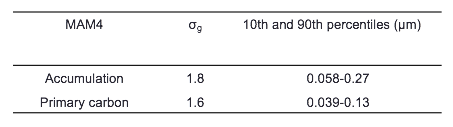
\includegraphics[width = 0.7\textwidth]{Rplot01}
		\caption[]{\label{fig_P1} Parameters of Lognormal Distribution}
	\end{center}
\end{figure}

\noindent The mean BC core diameter in accumulation mode is estimated as:
\begin{align*}
D_{\text{core}} = (D_{\text{mixed}}^3 \times f_{\text{BC}})^\frac{1}{3} 
\end{align*}
, where $D_{\text{core}}$ is the mean diameter of BC core,$D_{\text{mixed}}$ is the mean diameter of internally mixed particles (\textbf{extracted from model}), and $f_{\text{BC}}$ is the volume fraction of BC in accumulation mode.



 
\section{Compute Volume Fraction Corresponding to Lognormal Distribution}

The CDF of number distribution in the size range between $d_{1}$ and $d_{2}$ is:
\begin{align*}
N(\text{d}_{1}, \text{d}_{2}) = \frac{1}{\text{ln}\sigma_{\text{g}}\sqrt{2\pi}}\int_{d_{1}}^{d_{2}}e^-\frac{(\text{lnr} - \text{lnr}_{g})^2}{2\text{ln}^2\sigma_{\text{g}}}\text{d}(\text{lnr})
\end{align*}
, where $r_{g}$ is mean geometric diameter (extracted from model, varying temporally and spatially). 

\noindent The mean volume is proportional to function of the form:
\begin{align*}
N(\text{d}_{1}, \text{d}_{2}) &= \frac{1}{\text{ln}\sigma_{\text{g}}\sqrt{2\pi}}\int_{d_{1}}^{d_{2}}r^3e^-\frac{(\text{lnr} - \text{lnr}_{g})^2}{2\text{ln}^2\sigma_{\text{g}}}\text{d}(\text{lnr})  \\
&=\frac{e^{\frac{k^2}{2}ln^2\sigma_{g}+klnr_{g}}}{\text{ln}\sigma_{\text{g}}\sqrt{2\pi}}\int_{d_{1}}^{d_{2}}r^3e^-\frac{(\text{lnr} - \text{lnr}_{\text{gv}})^2}{2\text{ln}^2\sigma_{\text{g}}}\text{d}(\text{lnr})
\end{align*}
, where the volume mean diameter is of the form $\text{lnr}_{\text{gv}} = \text{lnr}_{\text{g}} + 3\text{ln}\sigma_{\text{g}}$.

\noindent So BC mass fraction (in the size range between 90 and 400 nm) in each mode (Figure~\ref{fig_P2}) is derived by:

\begin{align*}
F(\text{d}_{1}, \text{d}_{2}) &= \frac{\frac{1}{\text{ln}\sigma_{\text{g}}\sqrt{2\pi}}\int_{d_{1}}^{d_{2}}r^3e^-\frac{(\text{lnr} - \text{lnr}_{g})^2}{2\text{ln}^2\sigma_{\text{g}}}\text{d}(\text{lnr})}
{\frac{1}{\text{ln}\sigma_{\text{g}}\sqrt{2\pi}}\int_{0}^{+\infty}r^3e^-\frac{(\text{lnr} - \text{lnr}_{g})^2}{2\text{ln}^2\sigma_{\text{g}}}\text{d}(\text{lnr})}  \\
&=\frac{\frac{e^{\frac{k^2}{2}ln^2\sigma_{g}+klnr_{g}}}{\text{ln}\sigma_{\text{g}}\sqrt{2\pi}}\int_{d_{1}}^{d_{2}}e^-\frac{(\text{lnr} - \text{lnr}_{\text{gv}})^2}{2\text{ln}^2\sigma_{\text{g}}}\text{d}(\text{lnr})}{\frac{e^{\frac{k^2}{2}ln^2\sigma_{g}+klnr_{g}}}{\text{ln}\sigma_{\text{g}}\sqrt{2\pi}}\int_{0}^{+\infty}e^-\frac{(\text{lnr} - \text{lnr}_{\text{gv}})^2}{2\text{ln}^2\sigma_{\text{g}}}\text{d}(\text{lnr})}\\
&=\frac{1}{\text{ln}\sigma_{\text{g}}\sqrt{2\pi}}\int_{d_{1}}^{d_{2}}e^-\frac{(\text{lnr} - \text{lnr}_{\text{gv}})^2}{2\text{ln}^2\sigma_{\text{g}}}\text{d}(\text{lnr}) \\
&=\frac{1}{2}[\text{erf}(\frac{\text{lnd}_{2} - \text{lnr}_{\text{gv}}}{\sqrt{2}\text{ln}\sigma})-\text{erf}(\frac{\text{lnd}_{1} - \text{lnr}_{\text{gv}}}{\sqrt{2}\text{ln}\sigma})]
\end{align*}

\begin{figure}[!h] 
	\begin{center}
		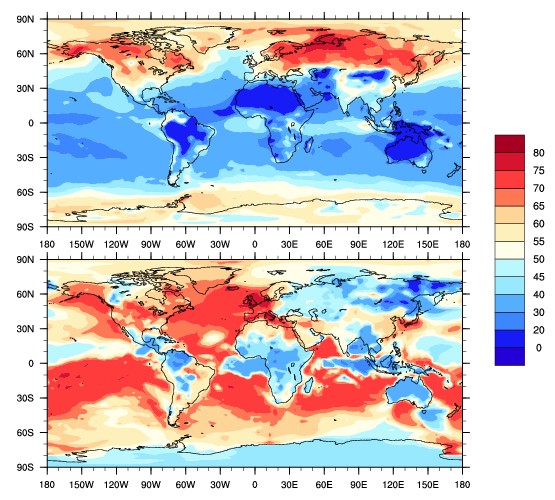
\includegraphics[width = 0.6\textwidth]{Rplot02}
		\caption[]{\label{fig_P2} BC mass fraction ($\%$) (between 90 and 400 nm) in primary carbon mode (top) and in accumulation mode (bottom), for surface layer, March.}
	\end{center}
\end{figure}


\noindent \textbf{Within the size range (90 to 400 nm)}, the ratio of BC mass in each mode to total BC mass is computed as:
\begin{align*}
f_{\text{accu}} = \frac{F_{\text{accu}}(\text{d}_{1}, \text{d}_{2})M_{\text{accu}}}{F_{\text{accu}}(\text{d}_{1}, \text{d}_{2})M_{\text{accu}}+F_{\text{pc}}(\text{d}_{1}, \text{d}_{2})M_{\text{pc}}}\\
f_{\text{pc}} = \frac{F_{\text{pc}}(\text{d}_{1}, \text{d}_{2})M_{\text{pc}}}{F_{\text{accu}}(\text{d}_{1}, \text{d}_{2})M_{\text{accu}}+F_{\text{pc}}(\text{d}_{1}, \text{d}_{2})M_{\text{pc}}}
\end{align*}
\[f_{\text{accu}} + f_{\text{pc}} = 1\]

\noindent , where $f_{\text{accu}}$ is the fraction of BC mass in accumulation mode, $f_{\text{pc}}$ is the fraction of BC mass in primary carbon mode (Figure~\ref{fig_P3}), $M_{\text{accu}}$ and $M_{\text{pc}}$ are BC mass in accumulation mode and primary carbon mode respectively.

\begin{figure}[!h] 
	\begin{center}
		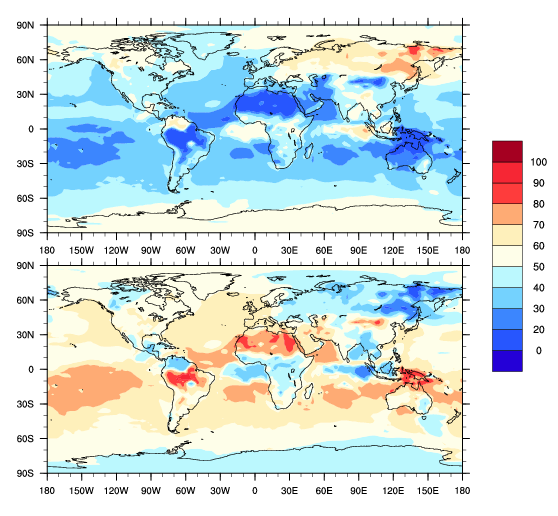
\includegraphics[width = 0.6\textwidth]{Rplot03}
		\caption[]{\label{fig_P3} Ratio of BC mass ($\%$) within SP2 size range to total BC mass within SP2 size range, in primary carbon mode (top) and accumulation mode (bottom), for surface layer, March.}
	\end{center}
\end{figure}











%%%%%%%%%%%%%%%%%%%%%%%%%%%%%%%%%%%%%%%%%%%%%%%%%%%%%%%%%%%%%%%%%%%%%%%%%%%%%%%%



\end{document}
%%%%%%%%%%%%%%%%%%%%%%%%%%%%%%%%%%%%%%%%%%%%%%%%%%%%%%%%%%%%%%%%%%%%%%%%%%%%%%%%
%%%%%%%%%%%%%%%%%%%%%%%%%%%%%%%%%%%%%%%%%%%%%%%%%%%%%%%%%%%%%%%%%%%%%%%%%%%%%%%%